% !TeX root = Report.tex
\section{Predicates}

When considering how to evaluate predicates there are many points that need to be considered. Depending on what the intention is certain implementations of predicate evaluation are going to be better than other implementations. Also, when developing with considerations of the predicate evaluation such as accuracy, the considerations of sensor networks will need to be taken into account (such as the minimisation of energy usage). This section will first detail the types of predicates that we identify that we wish to be able to detect, then it will cover how we can evaluate such predicates and finally will discuss several implementations of transmitting the information to the required part of the network.

\subsection{Types of Predicates}

In the introduction several different classes of predicates were discussed, of which the most important one is the locality of the predicate. A majority of the work focuses on global predicates \cite{277788,345831,553309} which while useful in general for distributed systems is perhaps not as helpful for wireless sensor networks. To begin with many of the problems that a sensor network may encounter are local problems. By local we mean that a node in the network only has access to a specific subset of the networks information, in our case we focus on the surrounding neighbours of the node evaluating the predicate. When forcing a local problem to be evaluated globally it means that investigating evaluating that predicate locally is eliminated. This is problematic as there may be energy savings when evaluating a predicate locally. So the first major decision is that instead of focusing on global predicates, local predicates are instead the focus - in order to investigate any potential energy savings.

\begin{mydef}
\emph{Global Predicate}: A predicate $P$ that operates on some global state $S$ where $S$ is a mapping from a node id to some data on that node.
\end{mydef}

\begin{mydef}
\emph{Local Predicate}: A predicate $P$ evaluated on the node $j$, where the state $N(n) \subseteq S$ available contains information on some $n$-hop neighbourhood of $j$.
\end{mydef}

The second decision is to decide on is the stability of the predicate being detected. As discussed in the introduction there is a choice between stable predicates that remain true and unstable predicates whose truth value can alternate. This decision is important because it will affect the algorithm structure, an example of this is that taking snapshots of global state and checking the predicate against that works for checking stable predicates. However, for unstable predicates detailed recording of the traces of the system is required \cite{bansod2004distributed}. Due to the limited resources of sensor nodes we focus on the simpler problem of stable predicates. This is mainly because complex programs tend to require a greater number of instructions to do more things and the size of the firmware on the motes is limited \cite{CM5000}.


\begin{mydef}
\emph{Application Predicate}: A predicate that is evaluated over the state an application is in. This can involve extracting and examining sensor data or program variables.
\end{mydef}

\begin{mydef}
\emph{Network Predicate}: A predicate that is evaluated over the network interactions. Examples include detecting collisions where there should have been none, or checking that there are no loops in multi-hop communications.
\end{mydef}

So far traditional predicate properties have been focused on. However, we need to introduce two new classes of predicates. In previous work the authors dealt in the abstract notion of program traces, these traces are simply events that lead to some eventual state. When developing software for sensor networks we feared that (i) the hooks to detect the traces and (ii) record them would be too demanding on the limited resources. By considering what happens in the application separately from the network the impacts may be decreased. Network predicates would involve monitoring the low level MAC layer for network events and also including extra data to packets sent from the node. Application predicates could imply be evaluated instantaneously on the data available. Due to the simplicity, but the good results that application predicates may provide we focus solely on them.

Much of the previous work exists in ideal worlds were assumptions such as ``no messages are lost'' \cite{277788} are made. Unfortunately this is not the case in the real world, while the MAC layer and the application layer can do much to mitigate packet loss \cite{?} without energy expensive protocols such as 802.11 \cite{?} it is not possible to eliminate packet loss. Therefore it must be realised that every time a predicate is evaluated it will have a certain level of accuracy. This is because some data may have been lost on the way to its destination or outdated information was used. We believe the accuracy is a very important angle to predicate evaluation as an accurate predicate evaluation that is not received often will inform the systems user more than a predicate evaluation result that is received very frequently but is also very inaccurate.

In summary we focus on evaluating predicates that are stable and use local information. These predicates also deal excursively with information about the application running on the mote and not the communication it is involved with. Also there should be a focus that predicates are evaluated as accurately as possible with a minimum amount of energy.

\subsection{Predicate Evaluation}


\subsubsection{Desired Features}

\begin{enumerate}
	\item Numerical support (Integer and Floating point) ($+$ $-$ $\times$ $/$ $=$ $\neq$ $<$ $\leq$ $>$ $\geq$)
	\item Set support (Creation and operating on) ($\cup$ $\cap$ $\setminus$ $\{\}$ $\forall$ $\exists$)
	\item Limited function support (eg. $Neighbourhood(N, H)$)
	\item Limited structure support (eg. $N.Temperature$)
	\item Ability to specify predicate target(s) (Single node, multiple nodes or entire network)
	\item Ability to get the current node ($this$)
	\item Ability to get sensor information on a node (temperature, humidity, \ldots)
	\item Ability to get node information (Distance to Sink, \ldots)
\end{enumerate}

\subsubsection{Non-Required Features}

There are lots of features that are usually provided by scripting languages that would cause undesirable effects such as inflating the binary size.

\begin{enumerate}
	\item Strings
	\item Complicated data structures (Lists, Arrays, Dictionaries, \ldots)
	\item Library features (Custom libraries or built-in libraries)
	\item Interactive mode (terminals)
	\item IO
\end{enumerate}



\subsection{Data Transmission}




\subsubsection{Evaluation Methods}

\begin{enumerate}
	\item Send scripting language to node, they interpret and evaluate it
	\item Compile predicate on base station, compress and send to node(s) for evaluation
\end{enumerate}

\subsubsection{Scripting Languages Considered}

\begin{enumerate}
	\item eLua \url{http://www.eluaproject.net/} \cite{elua}
	\item SCript \url{http://www.sics.se/~adam/dunkels06lowoverhead.pdf} \cite{dunkels06lowoverhead}
	\item wren \url{https://github.com/darius/wren} \cite{wren}
	\item Write the predicate in C, compile it to machine code and send it to the nodes to be evaluated
	\item \url{http://dunkels.com/adam/tsiftes11database.pdf} Antelope
\end{enumerate}


\subsection{Where to Evaluate Predicates}

Given the problem of assigning slots in a TDMA MAC protocol, one would wish to ensure that no node within two hops of any given node has the same slot. This raises a question of where this predicate should be evaluated to ensure minimum energy usage in its evaluation.

The first predicate we might consider is the one where for ever node, we get the 2-hop neighbourhood and check that none of those nodes have the same slot as the initial node. This means that we would need to send:
\begin{enumerate}
	\item A message from the base station to the node asking it to evaluate the predicate
	\item A message from the node to each of its 2-hop neighbours
	\item Each 2-hop neighbour needs to send a message back to the node
	\item The node would need to wait for its neighbours to send the messages, then evaluate the predicate. This would imply that the node would need to know who is in its two hop neighbourhood
	\item The node would need to report to the base station the result of the predicate
\end{enumerate}

So we would need at best $2\Delta_{sink} + 2|Neighbours(n, 2)|$ messages to evaluate this predicate for one node.

\begin{align}
\label{eq:2-hop-slot-pred}
& \hspace{3em}	\forall n \in Nodes \cdot \\
& \hspace{6em}		\forall n' \in Neighbours(n, 2) \cdot \\
& \hspace{9em}			(n.slot \neq n'.slot)
\end{align}

The second predicate we could consider is the one where every node checks their 1-hop neighbourhood for slot collisions. Here we model the 2-hop nature of the predicate differently, because instead of checking on the node that we want to check for slot collisions, we check on the node between two nodes that might have slot collisions.

\begin{enumerate}
	\item A message from the base station to the node adjacent to that we asking to check slot collisions
	\item A message from the node to each of its 1-hop neighbours
	\item Each 1-hop neighbour needs to send a message back to the node
	\item The node would need to wait for its neighbours to send the messages, then evaluate the predicate. This would imply that the node would need to know who is in its two hop neighbourhood
	\item The node would need to report to the base station the result of the predicate
\end{enumerate}

So we would need at best $2(\Delta_{sink} + 1) + 2|Neighbours(n, 1)|$ messages to evaluate this predicate for one node.

\begin{align}
\label{eq:1-hop-slot-pred}
&				\forall n \in Nodes \cdot \\
& \hspace{3em}		\forall n' \in Neighbours(n, 1) \cup \{n\} \cdot \\
& \hspace{6em}			\forall n'' \in Neighbours(n, 1) \cup \{n\} \cdot \\
& \hspace{9em}				(n' \not= n'' \implies n'.slot \neq n''.slot)
\end{align}

Overall we can assume that $|Neighbours(1, n)| \leq |Neighbours(2, n)|$, so checking 1-hop neighbours would in general require fewer message. Also we can assume that when checking these predicates, we would make sure that every node is checked (as the predicates are defined). This means that the first predicate would duplicate the checks: checking node $n$ for a collision with $n'$ and when $n'$ is asked to check the predicate it will query $n$.

However, if we were not asking the entire network to check for this property, then the first predicate would behave better. This is because the second predicate would have to be called for every 1-hop neighbour of the intended node. However, as it is assumed that the entire network would be asked if this predicate holds, then the second predicate is better.


\subsubsection{Getting and Waiting for Neighbourhood Data}

\begin{enumerate}
	\item If all neighbours are known then 1-hop predicates can wait for each node to send data. This has extra memory and communication requirements
	\item If we do not know who our n-hop neighbours are then we can just set a time out to wait for results
	\begin{enumerate}
		\item If we do not receive all items what should be done?
		\item Should we report that the predicate is true, even though we didn't receive all the information?
	\end{enumerate}
	\item What data should be sent from surrounding nodes and how could we access it?
\end{enumerate}


When asking for information on the neighbourhood, it possible to consider optimisations due to the structure of the predicate. For example take conjunctive predicates where the structure of the predicate $P$ is $P = P_1 \land P_2 \land \ldots \land P_n$. If one of the $P_i$ is false then the result of the predicate $P$ is false ($False \land P \Leftrightarrow False$). This means that the statements could potentially be evaluated in an order such that the $P_i$ that requires the fewest resources is evaluated first and the $P_j$ that requires the most resources is evaluated last.

The aim of this optimisation is to reduce energy usage by sending fewer messages. For the two types of data gathering in-network and at the sink, when gathering this data at the sink it would not be of any use as the data is sent to the sink in an event-based or periodic way. The sink doesn't ask for this information, so it is not possible for it to not ask for certain pieces of data. This is also true of event-based in-network predicate checking. So the only time this optimisation would be of use to us is when gathering data for in-network predicates that are checked periodically.

Surprisingly, asking for and receiving all the required information actually requires fewer messages than incrementally asking for information. This is because of the communication that needs to be repeated when asking for more information. For example if you have a conjunctive predicate where the sub-predicates require 1 and 3 hops of information. If we ask for all information then we simply send messages out 3 hops and then receive replies from all the nodes in that neighbourhood. If we instead ask for one-hop information first and then three-hop, we first have to send a message to local neighbours and then will end up sending them another data request message when asking for three-hop information (as the 1-hop neighbourhood is contained within the 3-hop neighbourhood).

For some predicates it may make obvious sense, such as if there is a conjunctive predicate that needs 1-hop information and 15-hop information. If the 1-hop predicate is often false, then it saves asking for information from all nodes that are within 15 hops of the evaluating node. However, as many of the predicates are not likely to require information from that distance (we expect one to two hops, with the possibility of three hops) it is an optimisation that would end up degrading the performance of requesting the near-by information. Also adding this feature would increase the firmware size, which began to reach the limit when the predicate evaluation libraries that aggregate data to the sink were implemented.

% Include equations if someone can be bothered to work them out
\begin{comment}
\begin{figure}[H]
\begin{equation}
\sigma(x) = \sum_{i=1}^{x} i \times |N(i)|
\end{equation}
\caption{The number of messages required to respond x hops}
\end{figure}

The sigma function is defined as it is because for each of the nodes that are $x$ hops away they will require sending their data message $x$ hops to reach the requesting node.

\begin{figure}[H]
\begin{equation}
\sum_{j \in H} j + \sigma(j)
\end{equation}
\caption{Maximum number of messages for an incremental data request}
\end{figure}

\begin{figure}[H]
\begin{equation}
|N_F(\text{max}(H))| \times \text{max}(H) + \sigma(\text{max}(H))
\end{equation}
\caption{Number of messages for a complete data request}
\end{figure}
\end{comment}


\subsection{Implementing Primitives}

There are certain primitives that we are going to need to implement. One of these is the $Neighbours(n, h)$ primitive, that takes a parameter $n$ that is the node we wish to get neighbour information on and $d$ which is the distance in hops from the node $n$ that we will ask for information.

\begin{align}
\label{eq:hcluster-neighbours-predicate}
& \hspace{3em}	\forall n \in Nodes \cdot \\
& \hspace{6em}		\exists n' \in Neighbours(n, H) \cdot \\
& \hspace{9em}			IsClusterHead(n)
\end{align}

An example of a predicate that uses $Neighbours(n, h)$ is shown above. This predicate is for Hierarchical Clustering where $H$ is a parameter that defines the distance between cluster heads. The predicate checks that for every node there is a neighbour in the $H$-hop neighbourhood that is a cluster head.

An alternative way that we might specify this predicate is to check that the distance between a node and the cluster head (that it knows the address of) is within $H$ hops.

\begin{align}
\label{eq:hcluster-distance-predicate}
& \hspace{3em}	\forall n \in Nodes \cdot \\
& \hspace{6em}		IsSink(n) \lor Distance(n, ClusterHead(n)) \leq H
\end{align}

However, there is an issue with this predicate. How would we implement the $Distance(n, n')$ primitive? With $Neighbours(n, h)$ we know how far we need to ask for information ($h$ hops), with $Distance(n, n')$ the maximum distance that we will need to wait for information to return from is the diameter of the network. Unfortunately we cannot assume that the diameter is known. If instead we take a time-out approach there is no way that we can guarantee to wait for the correct amount of time. For example if we wait enough time to check if a node is at maximum $D$ hops from the given node the node will need to wait for $2 \times D \times T_{send}$ time units. However, if the node we are trying to find the distance of is at $D + 1 $ hops then we will not believe the two nodes are connected. To reliably wait to check if two nodes are connected in a network where the diameter is not known we will need to wait for $\infty$ time units. Thus making $Distance(n, n')$ impossible to implement without knowing the diameter.


\subsection{Response to Predicate Evaluation}

Once a node has reached the point of having a result after evaluating a predicate it needs to do something meaningful with that information so that users looking for results at the base station also end up knowing this information. The first and most obvious solution would be to inform the base static of every result, be it success or failure. Unfortunately while this is the most comprehensive response it is would also require the most energy as every node would need to send a repose message for every predicate they were evaluating ($C = |P_{all}| \times |V| + |P_{single}|$).

The alternatives are to either send a message when a predicate has failed or when a predicate succeeds. This allows only a fraction of $C$ messages to be sent. However, there are a number of differences that make deciding to send success or failure an important decision. First of all is how the result is represented. The comprehensive solution has the advantage that the result of a predicate can be put into an \emph{unknown} state. Once a result message is received the result of that predicate can be moved into a \emph{failed} or \emph{succeeded} state. For success or failure messages you would need to assume the opposite of the messages that you are waiting for (i.e. assume predicates failed before receiving the succeeded message and vice versa) and change the state once the message is received. If messages are lost then this will lead to false notifications of success when waiting for failure messages and false failures when waiting for success messages.

The other issue to consider is what should be reported. If success messages are the chosen form of the response, then what useful information could they contain? One would expect the state that the predicate was evaluated with, but this information is not nearly as useful as the state that caused a predicate to fail. Another factor is that to create a useful description of why an error message failed is complex and would require more resources than simply evaluating the message. This means that practically it would be best for a failure message to report the state that caused the predicate to fail back to the base station and then expect further analysis on it there.

As we expect a predicate failure to be an infrequent event, our libraries have been designed to report only predicate failures. This should save energy in the form of messages. However, we expect the system to be vulnerable to not showing the full extent failures (falsely appearing successful), when messages are lost.


\subsection{Domain Specific Language}

\subsubsection{Definition}
\begin{eqnarray*}
	\pn{eval} & \pp & [ \pn{target} ] \ww \pn{using} \\
	\pn{target} & \pp & \sm{all} \\
	~ & \oo & \pn{number}\sm{.}\pn{number} \\
%
	\pn{using} & \pp & \sm{using} \ww \sm{Neighbours}\sm{(}\pn{number}\sm{)} \ww \sm{as} \ww \pn{variable} \ww \sm{in} \ww \pn{using} \\
	~ & \oo & \pn{predicate} \\
%
	\pn{predicate} & \pp &  \sm{(}\pn{predicate}\sm{)} \\
	~ & \oo & \pn{quantifier}\sm{(}\pn{variable} \ww \sm{:} \ww \pn{variable} \ww \sm{\mytilde} \pn{predicate} \sm{)}\\
	~ & \oo &  \pn{predicate} \ww \pn{logical-binary} \ww \pn{predicate} \\
	~ & \oo &  \pn{logical-unary} \ww \pn{predicate} \\
	~ & \oo &  \pn{var-expr} \ww \pn{math-logical-binary} \ww \pn{var-expr} \\
%
	\pn{var-expr} & \pp & \sm{(}\pn{var-expr}\sm{)} \\
	~ & \oo & \pn{variable} \\
	~ & \oo & \pn{number} \\
	~ & \oo & \pn{string}\sm{(}\pn{this-variable}\sm{)} \\
	~ & \oo & \pn{var-expr} \ww \pn{math-binary} \ww \pn{var-expr} \\
	~ & \oo & \sm{abs}\sm{(}\pn{var-expr}\sm{)} \\
	~ & \oo & \pn{set-fn}\sm{(}\pn{variable}\sm{)} \\
	~ & \oo & \pn{transform-set-fn}\sm{(}\pn{transform-fn}\sm{,} \ww \pn{variable}\sm{)} \\
%
	\pn{this-variable} & \pp & \pn{variable} \oo \sm{this} \\
	\pn{variable} & \pp & \pn{string} \\
%
	\pn{transform-fn} & \pp & \pn{string} \\
	\pn{transform-set-fn} & \pp & \sm{sum} \oo  \sm{mean} \oo \sm{max} \oo \sm{min} \\
	\pn{set-fn} & \pp & \sm{len} \\
%
	\pn{logical-binary} & \pp & \sm{\&}  \oo \sm{\textbar} \oo \sm{\textasciicircum} \oo \sm{=\textgreater} \oo \sm{\textless=\textgreater} \\
	\pn{logical-unary} & \pp & \sm{!} \\
	\pn{math-logical-binary} & \pp & \sm{==} \oo \sm{!=} \oo \sm{\textless} \oo \sm{\textless=} \oo \sm{\textgreater} \oo \sm{\textgreater=} \\
	\pn{math-binary} & \pp & \sm{+} \oo \sm{-} \oo \sm{*} \oo \sm{/} \oo \sm{**} \oo \sm{\%} \\
%
%	\pn{string} & \pp & \pn{alpha}\pn{string-rest} \\
%	\pn{string-rest} & \pp & \nn \oo \pn{alpha}\pn{string-rest} \oo \pn{digit}\pn{string-rest} \\
%
%	\pn{alpha} & \pp & \sm{A}\dots\sm{Z} \oo \sm{a}\dots\sm{z} \\
%	\pn{number} & \pp & \pn{sign} \pn{number-first} \oo \pn{number-first} \\
%	\pn{number-first} & \pp & \pn{digit} \oo \sm{1}\dots\sm{9}\pn{number-rest} \\
%	\pn{number-rest} & \pp & \pn{digit} \oo \pn{digit}\pn{number-rest} \\
%	\pn{digit} & \pp & \sm{0}\dots\sm{9} \\
%	\pn{sign} & \pp & \sm{+} \oo \sm{-} \oo \nn \\
	\pn{quantifier} & \pp & \sm{@} \oo \sm{\#} \\
\end{eqnarray*}

\textbf{TODO: Add float expansions}

used \url{http://cs.lmu.edu/~ray/notes/javacc/} and \url{http://www.engr.mun.ca/~theo/Misc/exp_parsing.htm} to get infix operator parsing working

\subsubsection{Examples}

\begin{figure}[H]
\begin{verbatim}
using Neighbours(2) as twohopn in
    @(x : twohopn ~
        slot(x) != slot(this)
    )
\end{verbatim}
\caption{Check that no two neighbours have the same slot (2-hop information)}
\label{fig:two-hop-slot-pred-lang}
\end{figure}

\begin{figure}[H]
\begin{verbatim}
using Neighbours(1) as onehopn in
    @(x : onehopn ~
        @(y : onehopn ~
            addr(x) != addr(y) => slot(x) != slot(y)
        ) & 
        slot(x) != slot(this)
    )
\end{verbatim}
\caption{Check that no two neighbours have the same slot (1-hop information)}
\label{fig:one-hop-slot-pred-lang}
\end{figure}

Predicates like those in \autoref{fig:two-hop-slot-pred-lang} and \autoref{fig:one-hop-slot-pred-lang} are found at \cite{DBLP:journals/corr/abs-0808-0920}.

\begin{figure}[H]
\begin{verbatim}
temperature(this) <= 40.0
\end{verbatim}
\caption{Check that our temperature is less than or equal to 40 degrees}
\end{figure}

\begin{figure}[H]
\begin{verbatim}
using Neighbours(2) as twohopn in
    abs(temperature(this) - mean(temperature, twohopn)) <= 10.0
\end{verbatim}
\caption{Check that the average neighbour temperature is with 10 degrees of ours}
\end{figure}


\begin{figure}[H]
\begin{verbatim}
using Neighbours(H(this)) as neighbours in
    #(node : neighbours ~
        ch(this) == addr(node)
    )
\end{verbatim}
\caption{Check cluster head is in H-hop neighbourhood}
\end{figure}



\begin{figure}[H]
\begin{verbatim}
using Neighbours(1) as onehopn in
    using Neighbours(2) as twohopn in
        @(a : onehopn ~
            #(b : twohopn ~ addr(a) == addr(b))
        )
\end{verbatim}
\caption{Check 1-hop neighbourhood is in 2-hop neighbourhood}
\end{figure}


\begin{figure}[H]
\begin{verbatim}
using Neighbours(1) as onehopn in
    base-station-distance(this) == min(base-station-distance, onehopn) + 1
\end{verbatim}
\caption{We are one hop further from the base station than the closest of our neighbours}
\end{figure}


\subsection{Virtual Machine}

\subsubsection{Opcodes}

\begin{verbatim}
_ is either I for int or F for float

For binary operations the order the operands are used is specified as x op x.
When x is 0 the value on the top of the stack is used. When x is 1 the
value after the one on the top of the stack is used.

HALT
    Halts execution.
    The stack should always have at least one integer on it when halting.

_PUSH (_)
    Pushes an _ onto the stack.

_POP
    Pops the stack by sizeof(_) bytes.

_FETCH (variable id - ubyte)
    Fetches the value of the given variable and pushes the
    first sizeof(_) bytes of it onto the stack.

_STORE (variable id - ubyte)
    Stores the first sizeof(_) bytes in the variable
    of the given name.

AFETCH (variable id - ubyte)
    Fetches the value of the array named in the parameter
    at the integer index at the top of the stack.

ALEN (variable id - ubyte)
    Pushes an integer onto the stack containing the length
    of the named array.
	
ASUM  (variable id - ubyte) (function id - ubyte)
AMEAN
AMAX
AMIN
    Over the user defined array stored in the variable whose
    name is the first parameter, transform it using the function
    whose name is the second parameter. On this transformed data
    calculate the array operation and push the result as a float
    onto the top of the stack.

CALL (function id - ubyte)
    Calls the named function on the data on top of the stack.
    Pop's the data that was given to the function off the top of
    the stack and pushes the result onto the top of the stack.

ICASTF
    Pops an integer off the stack, casts it to a float
    then stores it back on the stack.

FCASTI
    Pops a float off the stack, casts it to a integer
    then stores it back on the stack.

JMP (ubyte)
    Jumps to a position in the code relative to the start
    of the program.

JZ (ubyte)
    Pops and reads the top of the stack as an integer, if it is 0
    the program jumps to the location, otherwise evaluation
    continues.

JNZ (ubyte)
    Pops and reads the top of the stack as an integer, if it is not 0
    the program jumps to the location, otherwise evaluation
    continues

_ADD        1 op 0
_SUB        1 op 0
_MUL        1 op 0
_DIV1       0 op 1
_DIV2       1 op 0
    Performs a mathematical operations on the first two sizeof(_)
    values on the stack. Pops both values off the stack, stores
    the result in the same type back on the stack.

IINC
    Pops the top of the stack by sizeof(int) bytes, increments
    the value as an integer. Pushes the result back on the stack

_EQ	        1 op 0
_NEQ        1 op 0
_ILT        1 op 0
_LEQ        1 op 0
_GT	        1 op 0
_GEQ        1 op 0
    Performs a mathematical operations on the first two sizeof(_)
    values on the stack. Pops both values off the stack, stores
    the result in an integer on the stack.

AND         1 op 0
OR          1 op 0
XOR	        1 op 0
EQUIVALENT  1 op 0
IMPLIES     1 op 0
    Performs a logical operation on the first two values on the
    stack. These are not bitwise operations and the expected
    formats of the values are integers. 0 is false, 1 is true.
    Pops both values off the stack,
    stores the result in an integer back on the stack.

NOT
    Pops an integer off the stack, performs logical not on it.
    Pushes the result back on the stack.
	
_VAR (variable id - ubyte)
    Creates a variable of type _ with the id set to the given
    unsigned byte.
\end{verbatim}


\subsubsection{Bytecode}

One of the most important aims of the predicate language's bytecode was to be as small as possible. The reason for this was to support sending as much program information in the limited length of a network packet. To achieve this aim it meant that we needed to make the virtual machine handle more abstract representations of its components. For example, initially the bytecode for calling a function contained a byte for the opcode of \verb|CALL| and then a string of characters which contained the name of the function to call. At minimum this would cost 2 bytes - one for the character of the function's name and one for the NUL character. To improve this the string was replaced with a single byte, which means that the number of functions callable by the virtual machine ends up being limited to 256. The same was true for the variable ids as well and as the variable id is contained with an unsigned byte, they to are limited to 256.


When developing the virtual machine what also became important was the fact that the bytecode was a string of unsigned bytes, where sequences of them could end up representing a 16 bit integer or a 32 bit float. This is important because it could mean that we would try to perform unaligned reads which the CPU of our motes could potentially get wrong\footnote{\url{http://permalink.gmane.org/gmane.os.contiki.devel/1462}}, this is due to the restrictions the CPU has on the alignment of words ``Bytes are located at even or odd addresses. Words are only located at even addresses \ldots. When using word instructions, only even addresses may be used. The low byte of a word is always an even address'' \cite[Section~1.4.5 (p.~28)]{msp430usersguide}.

\begin{figure}[ht!]
\centering
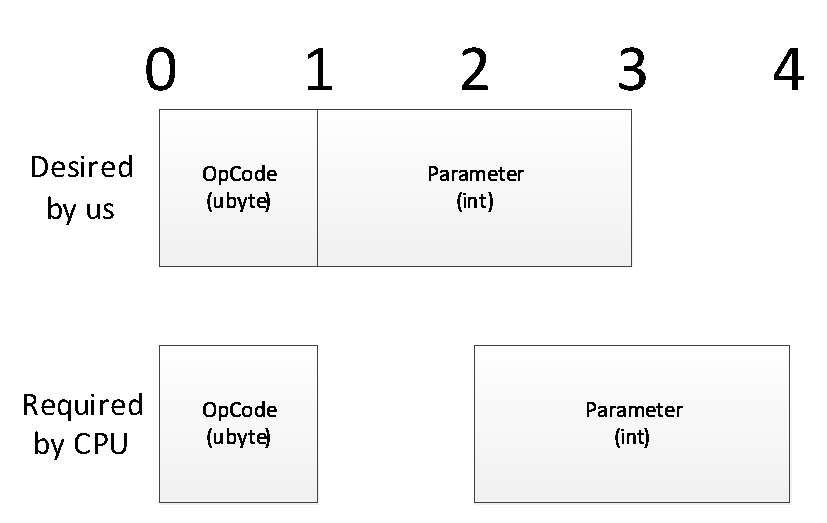
\includegraphics[scale=0.75]{Diagrams/byte-alignment.eps}
\caption{Alignment Issues}
\label{fig:alignment-issues}
\end{figure}

\begin{figure}[ht!]
\begin{verbatim}
[java] **** Illegal read - misaligned word from $2c01 at $80de
[java] Stack Trace: number of calls: 4 PC: $80de
[java] evaluate (errno.c) called from PC: $7166 (elapsed: 164446)
[java] process_thread_mainProcess (local in pred-eval.c) called from PC: $bf12 (elapsed: 536355)
[java] call_process (local in process.c) called from PC: $c0b2 (elapsed: 536391)
[java] process_run (errno.c) called from PC: $4250 (elapsed: 536996)
\end{verbatim}
\caption{Example of the error messages produced by MSPSim in Cooja that led to the discovery of this bug}
\end{figure}

As can be seen in \autoref{fig:alignment-issues} if we were to align the words as the CPU wanted the size of the bytecode would massively increase as every single byte bytecode would need to be padded by a byte to (i) make sure all bytecode entries were the same length and to ensure the word parameters are correctly aligned. To solve this issue instead of accessing the memory directly in the bytecode what can be done instead is to copy the memory out byte-by-byte into a correctly aligned block of memory and use that instead.

\subsection{Testing}

As the virtual machine and its parsers can be fairly complex and difficult pieces of code to understand it was very important that we had test cases that validated that the functionality was correct. To do this three sets of tests are performed. Of them two are unit tests, one that tests that assembled bytecode can be correctly executed and the other that tests that the parser can correctly parse and generate code. After this is an integration test, that checks if the output of the parser/compiler converted into bytecode by the assembler can be correctly executed. To test the correct execution set data is given to the virtual machine, which can then be used in the predicates.

Different things are tested for each of the integration tests. When testing the assembler and virtual machine, short programs of opcodes are provided to test simple activities such as pushing onto the stack, calling functions or arithmetic. This is simply to test the functionality of the virtual machine. As we can be sure that the functionality is correct, when testing the compiler more complex predicates that we have designed the system to use are tested. We expect that for some of these tests scripts the code would be the same for real world uses.
